

\pgfplotsset{%
    name nodes near coords/.style={
        every node near coord/.append style={
            name=#1-\coordindex,
            alias=#1-last,
        },
    },
    name nodes near coords/.default=coordnode
}


\pgfplotsset{/pgfplots/bar cycle list/.style={/pgfplots/cycle list={
            {olive,fill=olive!40!white,mark=none},
            {brown,fill=brown!40!white,mark=none},
            {teal,fill=teal!50!white,mark=none},
            {black,fill=gray,mark=none},},},}
            
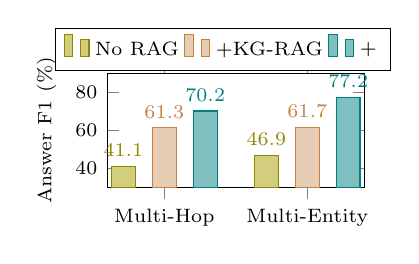
\begin{tikzpicture}
\tikzstyle{every node}=[font=\scriptsize]
    \begin{axis}[
            ybar=.22cm,
            bar width=.3cm,
            enlarge x limits={0.4},
            width=0.4\textwidth,
            height=0.25\textwidth,
            legend style={at={(.45,1.4)},
                anchor=north,legend columns=-1},
            symbolic x coords={ Multi-Hop, Multi-Entity},
            xtick=data,
            nodes near coords,
            nodes near coords align={vertical},
            ymin=30,ymax=90,
            compat=1.5, 
            ylabel={Answer F1 (\%)},
            ylabel near ticks,
        ]
\addplot+[name nodes near coords=bn] coordinates {(Multi-Hop,41.1)[{41.1}] (Multi-Entity,46.9)[{46.9}]};
 \addplot+[name nodes near coords=rn] coordinates {(Multi-Hop, 61.3)[{61.3}] (Multi-Entity,61.7)[{61.7}]};
 \addplot+[name nodes near coords=ln] coordinates {(Multi-Hop,70.2)[{70.2}] (Multi-Entity,77.2)[{77.2}]};

        \legend{No RAG,+KG-RAG,+\textbf{\grag}}
    \end{axis}


            
\end{tikzpicture}

